\documentclass[11pt,compress,t,notes=noshow, xcolor=table]{beamer}
\usepackage[]{graphicx}\usepackage[]{color}
% maxwidth is the original width if it is less than linewidth
% otherwise use linewidth (to make sure the graphics do not exceed the margin)
\makeatletter
\def\maxwidth{ %
  \ifdim\Gin@nat@width>\linewidth
    \linewidth
  \else
    \Gin@nat@width
  \fi
}
\makeatother

\newcommand{\citebutton}[2]{%
\beamergotobutton{\href{#2}{#1}}%
}

\newcommand{\blu}[1]{\textcolor{blue}{#1}}
\newcommand{\org}[1]{\textcolor{orange}{#1}}
\newcommand{\ques}{\textbf{\textcolor{red}{Question:  }}}
\newcommand{\questionssofar}{\begin{frame}\frametitle{Any questions?}\end{frame}}

\newcommand\warning{%
 \makebox[1.4em][c]{%
 \makebox[0pt][c]{\raisebox{.1em}{\scriptsize!}}%
 \makebox[0pt][c]{\color{red}\normalsize$\bigtriangleup$}}}%

\definecolor{fgcolor}{rgb}{0.345, 0.345, 0.345}
\newcommand{\hlnum}[1]{\textcolor[rgb]{0.686,0.059,0.569}{#1}}%
\newcommand{\hlstr}[1]{\textcolor[rgb]{0.192,0.494,0.8}{#1}}%
\newcommand{\hlcom}[1]{\textcolor[rgb]{0.678,0.584,0.686}{\textit{#1}}}%
\newcommand{\hlopt}[1]{\textcolor[rgb]{0,0,0}{#1}}%
\newcommand{\hlstd}[1]{\textcolor[rgb]{0.345,0.345,0.345}{#1}}%
\newcommand{\hlkwa}[1]{\textcolor[rgb]{0.161,0.373,0.58}{\textbf{#1}}}%
\newcommand{\hlkwb}[1]{\textcolor[rgb]{0.69,0.353,0.396}{#1}}%
\newcommand{\hlkwc}[1]{\textcolor[rgb]{0.333,0.667,0.333}{#1}}%
\newcommand{\hlkwd}[1]{\textcolor[rgb]{0.737,0.353,0.396}{\textbf{#1}}}%
\let\hlipl\hlkwb

\usepackage{framed}
\makeatletter
\newenvironment{kframe}{%
 \def\at@end@of@kframe{}%
 \ifinner\ifhmode%
  \def\at@end@of@kframe{\end{minipage}}%
  \begin{minipage}{\columnwidth}%
 \fi\fi%
 \def\FrameCommand##1{\hskip\@totalleftmargin \hskip-\fboxsep
 \colorbox{shadecolor}{##1}\hskip-\fboxsep
     % There is no \\@totalrightmargin, so:
     \hskip-\linewidth \hskip-\@totalleftmargin \hskip\columnwidth}%
 \MakeFramed {\advance\hsize-\width
   \@totalleftmargin\z@ \linewidth\hsize
   \@setminipage}}%
 {\par\unskip\endMakeFramed%
 \at@end@of@kframe}
\makeatother

\definecolor{shadecolor}{rgb}{.97, .97, .97}
\definecolor{messagecolor}{rgb}{0, 0, 0}
\definecolor{warningcolor}{rgb}{1, 0, 1}
\definecolor{errorcolor}{rgb}{1, 0, 0}
\newenvironment{knitrout}{}{} % an empty environment to be redefined in TeX

\usepackage{alltt}
\newcommand{\SweaveOpts}[1]{}  % do not interfere with LaTeX
\newcommand{\SweaveInput}[1]{} % because they are not real TeX commands
\newcommand{\Sexpr}[1]{}       % will only be parsed by R
\newcommand{\xmark}{\ding{55}}%


\usepackage[english]{babel}
\usepackage[utf8]{inputenc}

\usepackage{dsfont}
\usepackage{verbatim}
\usepackage{amsmath}
\usepackage{amsfonts}
\usepackage{amssymb}
\usepackage{bm}
\usepackage{csquotes}
\usepackage{multirow}
\usepackage{longtable}
\usepackage{booktabs}
\usepackage{enumerate}
\usepackage[absolute,overlay]{textpos}
\usepackage{psfrag}
\usepackage{algorithm}
\usepackage{algpseudocode}
\usepackage{eqnarray}
\usepackage{arydshln}
\usepackage{tabularx}
\usepackage{placeins}
\usepackage{tikz}
\usepackage{setspace}
\usepackage{colortbl}
\usepackage{mathtools}
\usepackage{wrapfig}
\usepackage{bm}
\usepackage{amsmath}
\usepackage{pifont}

\usetikzlibrary{shapes.multipart,shapes,arrows,automata,positioning,calc,chains,trees, shadows}
\tikzset{
  %Define standard arrow tip
  >=stealth',
  %Define style for boxes
  punkt/.style={
    rectangle,
    rounded corners,
    draw=black, very thick,
    text width=6.5em,
    minimum height=2em,
    text centered},
  % Define arrow style
  pil/.style={
    ->,
    thick,
    shorten <=2pt,
    shorten >=2pt,}
}

\tikzstyle{vec}=[draw, rectangle, fill = white, minimum width=5mm, minimum height=1cm, inner sep = 2pt]

\usepackage{subfig}

% Defines macros and environments
\usepackage{../../style/lmu-lecture}


\let\code=\texttt
\let\proglang=\textsf

\setkeys{Gin}{width=0.9\textwidth}

\setbeamertemplate{frametitle}{\expandafter\uppercase\expandafter\insertframetitle}

\usepackage{bbm}
% basic latex stuff
\newcommand{\pkg}[1]{{\fontseries{b}\selectfont #1}} %fontstyle for R packages
\newcommand{\lz}{\vspace{0.5cm}} %vertical space
\newcommand{\dlz}{\vspace{1cm}} %double vertical space
\newcommand{\oneliner}[1] % Oneliner for important statements
{\begin{block}{}\begin{center}\begin{Large}#1\end{Large}\end{center}\end{block}}


%new environments
\newenvironment{vbframe}  %frame with breaks and verbatim
{
 \begin{frame}[containsverbatim,allowframebreaks]
}
{
\end{frame}
}

\newenvironment{vframe}  %frame with verbatim without breaks (to avoid numbering one slided frames)
{
 \begin{frame}[containsverbatim]
}
{
\end{frame}
}

\newenvironment{blocki}[1]   % itemize block
{
 \begin{block}{#1}\begin{itemize}
}
{
\end{itemize}\end{block}
}

\newenvironment{fragileframe}[2]{  %fragile frame with framebreaks
\begin{frame}[allowframebreaks, fragile, environment = fragileframe]
\frametitle{#1}
#2}
{\end{frame}}


\newcommand{\myframe}[2]{  %short for frame with framebreaks
\begin{frame}[allowframebreaks]
\frametitle{#1}
#2
\end{frame}}

\newcommand{\remark}[1]{
  \textbf{Remark:} #1
}


\newenvironment{deleteframe}
{
\begingroup
\usebackgroundtemplate{
\includegraphics[width=\paperwidth,height=\paperheight]{../style/color/red.png}}
 \begin{frame}
}
{
\end{frame}
\endgroup
}
\newenvironment{simplifyframe}
{
\begingroup
\usebackgroundtemplate{
\includegraphics[width=\paperwidth,height=\paperheight]{../style/color/yellow.png}}
 \begin{frame}
}
{
\end{frame}
\endgroup
}\newenvironment{draftframe}
{
\begingroup
\usebackgroundtemplate{
\includegraphics[width=\paperwidth,height=\paperheight]{../style/color/green.jpg}}
 \begin{frame}
}
{
\end{frame}
\endgroup
}
% https://tex.stackexchange.com/a/261480: textcolor that works in mathmode
\makeatletter
\renewcommand*{\@textcolor}[3]{%
  \protect\leavevmode
  \begingroup
    \color#1{#2}#3%
  \endgroup
}
\makeatother





\input{../../latex-math/basic-math.tex}
\input{../../latex-math/basic-ml.tex}
\newcommand*\POS[1]{\textsubscript{\texttt{#1}}} % tag with part of speech
\usepackage{qtree} %parse tree

\newcommand{\titlefigure}{figure/tasks.png}
\newcommand{\learninggoals}{
\item Understand the different types of tasks
\item Linguistic tasks vs. higher-level tasks}

\title{Basics}
% \author{}
\institute{\href{https://slds-lmu.github.io/lecture_dl4nlp/}{slds-lmu.github.io/lecture\_dl4nlp}}
\date{}

\begin{document}
\lecturechapter{NLP tasks}
\lecture{Deep Learning for NLP}

% ------------------------------------------------------------------------------

\begin{vbframe}{categorization of nlp tasks}

\vfill

\textbf{Distinction between:}

	\begin{itemize}
		\item Language modeling
		\item Token-level classification
		\item Sequence-level classification
		\item Similarity / Retrieval
		\item Text generation
	\end{itemize}
	
\vspace{.3cm}

\textbf{Connection to learning paradigms:}

	\begin{itemize}
		\item Given the task, some learning paradigms are more suitable
		\item Tasks can be formulated differently to fit a given learning paradigm
		\item Amount of available (labeled) data might depend on task
		\item Presence/Absence of labels important to consider
	\end{itemize}

\vfill

\end{vbframe}

% ------------------------------------------------------------------------------

\begin{vbframe}{language modeling}
	
\vfill

\textbf{Predict the next token:}

\begin{figure}
	\centering
		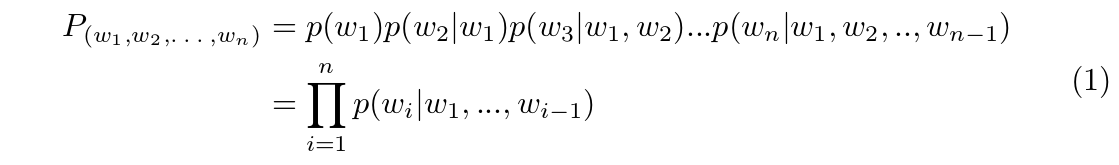
\includegraphics[width = 11cm]{figure/language-modeling.png}\\ 
		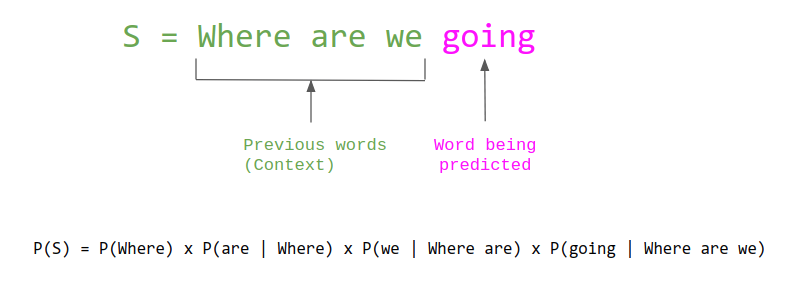
\includegraphics[width = 11cm]{figure/language-modeling2.png}\\
	\beamergotobutton{\href{https://thegradient.pub/understanding-evaluation-metrics-for-language-models/}{Source: The Gradient}}
\end{figure}

\vfill

\end{vbframe}

% ------------------------------------------------------------------------------

\begin{vbframe}{categorization of nlp tasks}

\vfill

\textbf{"Low-Level" tasks:}

	\begin{itemize}
		\item \textit{Token-level Classification}: Problems on a word/token level
		\item Modeling relationships \textit{between} words/tokens %(can also be rephrased to a token-level classification task)
		\item \textit{Note:} The latter one can also be formulated in such a way,\\that it can be solved as a \textit{token-level classification} task
	\end{itemize}
	
\vspace{.3cm}

\textbf{"High-Level" tasks:}

	\begin{itemize}
		\item \textit{Sequence-level Classification}: Problems on a sequence level
		\item \textit{Retrieval}: Assess (semantic) similarity on document-level
		\item Producing sequences of text based on an input sequences,\\known as \textit{seq2seq} tasks
		\item \textit{Note:} The latter one is also an instance of a generation task
	\end{itemize}

\vfill

\end{vbframe}

% ------------------------------------------------------------------------------

\begin{frame}{low-level: sequence tagging}

\vspace{1cm}

\textbf{POS-tagging (part of speech):}

\begin{exampleblock}{Example}
	Time flies   like   an   arrow.\\Fruit   flies   like   a   banana.
\end{exampleblock}

\vfill

\end{frame}

% ------------------------------------------------------------------------------

\begin{frame}[noframenumbering]{low-level: sequence tagging}

\vspace{1cm}

\textbf{POS-tagging (part of speech):}

\begin{exampleblock}{Example}
	Time flies   like   an   arrow.\\Fruit   flies   like   a   banana.
\end{exampleblock}

\begin{exampleblock}{Example}
		Time\POS{NN} flies\POS{VBZ}  like\POS{IN}   an\POS{DT}   arrow\POS{NN}.		\\ Fruit\POS{NN}   flies\POS{NN}   like\POS{VB}   a\POS{DT}   banana\POS{NN}.
\end{exampleblock}

\vspace{.5cm}

\begin{footnotesize}
IN = Preposition or subordinating conjunction (conjunction here); VBZ = Verb, 3rd person singular present; DT = determiner; NN = singular noun
\end{footnotesize}

\vfill

\end{frame}

% ------------------------------------------------------------------------------

\begin{frame}{low-level: structure prediction}
	
\vfill

\textbf{Chunking/Parsing:}

\begin{columns}[T,onlytextwidth]
\column{0.5\textwidth}

\begin{exampleblock}{Example}
\begin{scriptsize}
\Tree
[.S
	[.NP
		[.NN
			[ Time ]
		]
	]
	[.VP
		[.VBZ
			[ flies ]
		]
		[.PP
			[.IN
				[ like ]
			]
		]
		[.NP
			[.DT
				[ an ]
			]
			[.NN
				[ arrow ]
			]
		]
	]
]
\end{scriptsize}
\end{exampleblock}

\column{0.5\textwidth}

\begin{exampleblock}{Example}
	\begin{scriptsize}
\Tree
[.S
	[.NP
		[.NN
			[ Fruit ]
		]
		[.NN
			[ flies ]
		]
	]
	[.VP
		[.VB
			[ like ]
		]
		[.NP
			[.DT
				[ a ]
			]
			[.NN
				[ banana ]
			]
		]
	]
]
\end{scriptsize}
\end{exampleblock}
\end{columns}

\vfill
	
\end{frame}

% ------------------------------------------------------------------------------

\begin{frame}{low-level: semantics}

\vfill

\textbf{Word sense disambiguation:}

	\begin{exampleblock}{Example}
		Time flies   like   an   arrow. \hfil Fruit   flies   like   a   banana. \\
		
\includegraphics[width=0.3\linewidth]{figure/timeflies.png} \hspace{5.5em}
		
\includegraphics[width=0.3\linewidth]{figure/friutflies.png}
	\end{exampleblock}
	
\vfill

\end{frame}

% ------------------------------------------------------------------------------

\begin{frame}{Named Entity Recognition (NER)}

\vfill

\begin{exampleblock}{Example}
"... chancelor\POS{O} Angela\POS{B-PER} Merkel\POS{I-PER} said\POS{O} ..."
\end{exampleblock}

"BIO"-tagging
\begin{itemize}
	\item \texttt{B} = Begin of entity, e.g., \texttt{B-PER} (person), \texttt{B-LOC} (location)
	\item \texttt{I} = "Inside" entity, e.g, \texttt{I-PER}, \texttt{I-LOC}
	\item \texttt{O} = Other (no entity)
\end{itemize}
	
\vfill

\end{frame}

% ------------------------------------------------------------------------------

\begin{vbframe}{Token-level classification}

\vfill

\textbf{Pre-train/fine-tune:}

	\begin{figure}
		\centering
		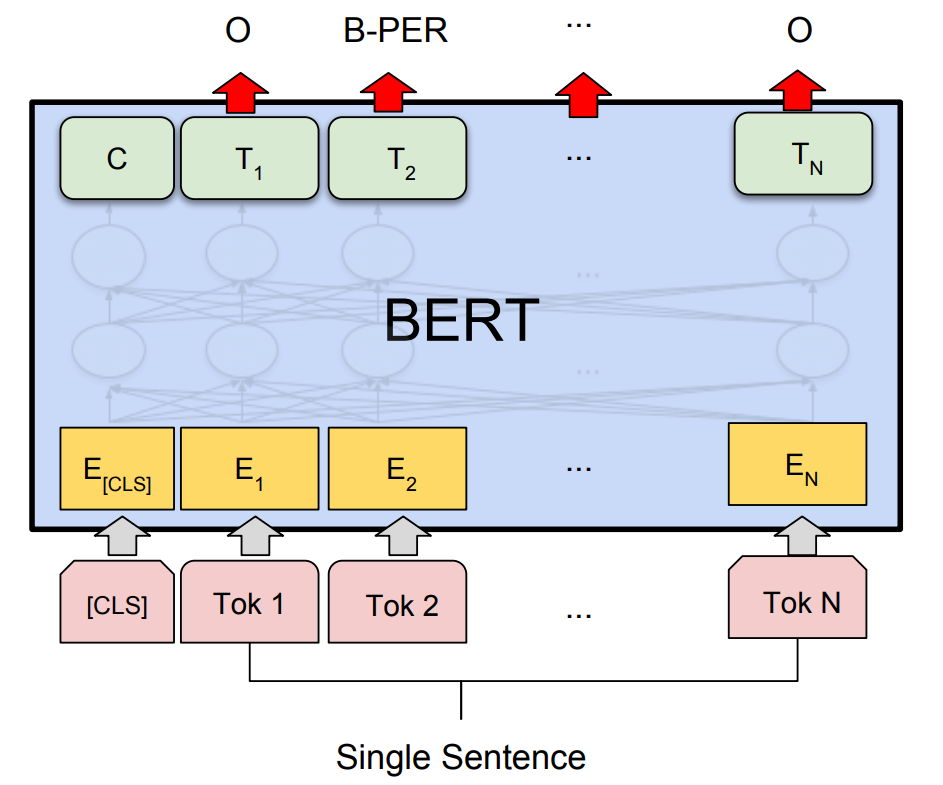
\includegraphics[width = 7cm]{figure/toklevel.png}\\ 
		\citebutton{Source: Devlin et al., 2019}{https://aclanthology.org/N19-1423.pdf}
	\end{figure}

\vfill

\end{vbframe}

% ------------------------------------------------------------------------------

\begin{frame}{high-level NLP tasks}

\vfill

\begin{itemize}
	\item \textbf{Information Extraction}
	\begin{itemize}
		\item search, event detection, textual entailment
	\end{itemize}
	\item \textbf{Writing Assistance} 
	\begin{itemize}
		\item spell checking, grammar checking, auto-completion
	\end{itemize}
	\item \textbf{Text Classification}
	\begin{itemize}
		\item spam, sentiment, author, plagiarism
	\end{itemize}
	\item \textbf{Natural language understanding} 
	\begin{itemize}
		\item metaphor analysis, argumentation mining, question-answering
	\end{itemize}
	\item \textbf{Natural language generation}
	\begin{itemize}
		\item summarization, tutoring systems, chat bots
	\end{itemize}
	\item \textbf{Multilinguality}
	\begin{itemize}
		\item machine translation, cross-lingual information retrieval
	\end{itemize}
\end{itemize}

\vfill

\end{frame}

% ------------------------------------------------------------------------------

\begin{vbframe}{sequence-level classification}

\vfill

	\begin{figure}
		\centering
		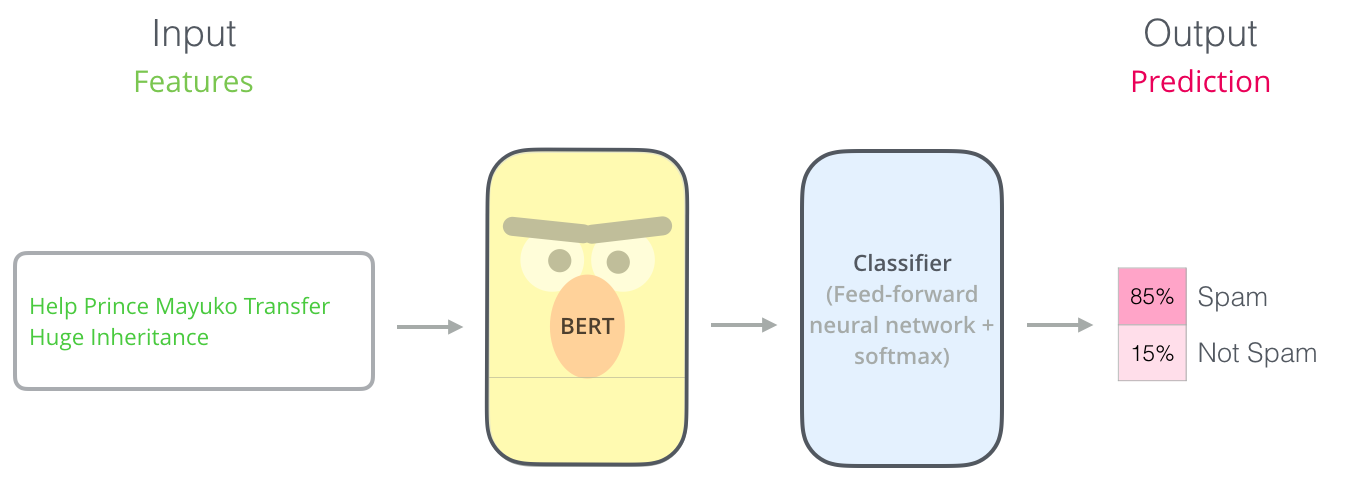
\includegraphics[width = 9cm]{figure/seqlevel.png}\\ 
		\beamergotobutton{\href{https://jalammar.github.io/illustrated-bert/}{Source: Jay Alammar}}
	\end{figure}
	
\textbf{Notes:}

\begin{itemize}
	\item BERT is a popular model, no need to know further details now 
	\item Output can also be non-binary, i.e. multi-class/-label 
\end{itemize}

\vfill

\end{vbframe}

% ------------------------------------------------------------------------------

\begin{vbframe}{sequence-level classification}

\vfill

\textbf{Reformulation as generative task:}

	\begin{figure}
		\centering
		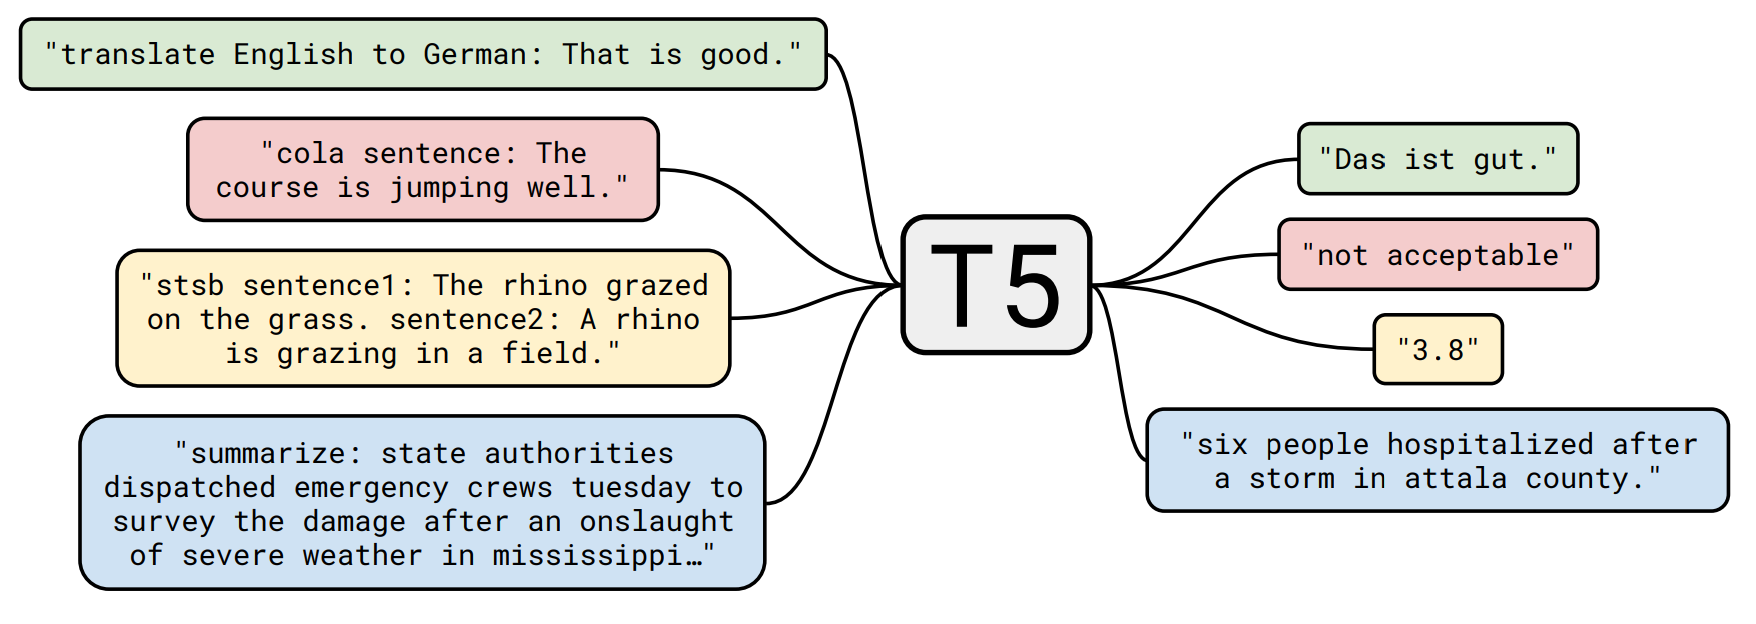
\includegraphics[width = 11cm]{../chapter06-t5/figure/t5.png}\\ 
		\beamergotobutton{\href{https://jmlr.org/papers/v21/20-074.html}{Source: Raffel et al., 2020}}
	\end{figure}

\vfill

\end{vbframe}

% ------------------------------------------------------------------------------

\begin{frame}{retrival (cf. previous chapter)}
	
\vfill

\textbf{Document retrieval}

\begin{figure}
	\centering
		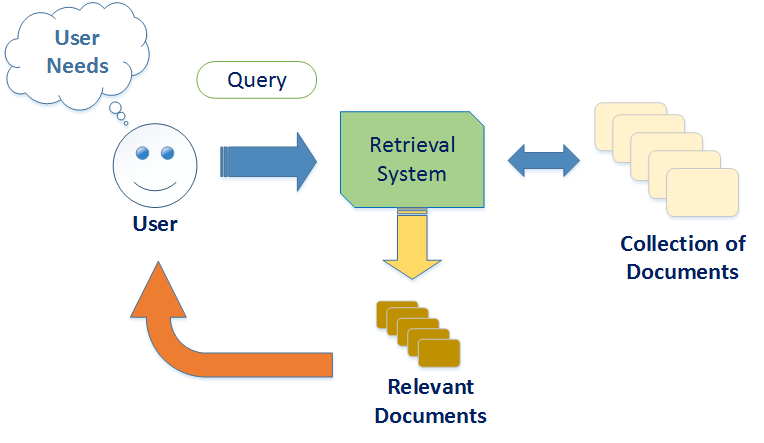
\includegraphics[width = 9cm]{figure/retrieval.png}\\ 
	\beamergotobutton{\href{https://www.analyticsvidhya.com/blog/2022/02/search-engines-using-deep-learning/}{Source: Analytics Vidhya}}
\end{figure}

\vfill

	
\end{frame}

% ------------------------------------------------------------------------------

\begin{vbframe}{generation: machine translation}

\vfill

\textbf{A brief History of Machine Translation}

\begin{itemize}
	\item Rule-Based Machine Translation (50s -- 80s)
		\begin{itemize}
			\item Dictionaries + Grammatical Rules
		\end{itemize}
	\item Example-Based Machine Translation (80s -- 90s)
		\begin{itemize}
			\item First suggested by Makoto Nagao (1984)
			\item Based on bilingual text corpora
		\end{itemize}
	\item Statistical Machine Translation (90s -- 10s)
		\begin{itemize}
			\item Driven by IBM guys
		\end{itemize}
	\item Neural Machine Translation (10s -- now)
		\begin{itemize}
			\item Based on neural networks (LSTMs, Transformers)
		\end{itemize}
\end{itemize}

\vfill

\end{vbframe}

% ------------------------------------------------------------------------------

\begin{vbframe}{Seq2Seq modeling}

\vspace{1cm}

	\begin{figure}
		\centering
		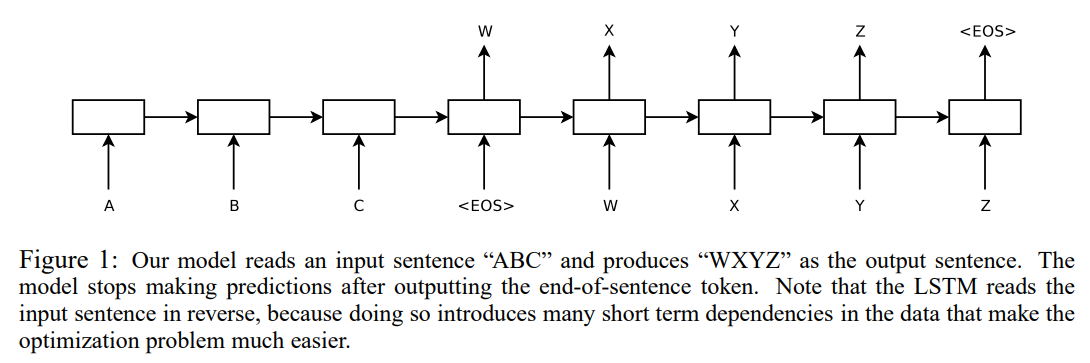
\includegraphics[width = 11cm]{figure/seq2seq.png}\\ 
	\beamergotobutton{\href{https://arxiv.org/pdf/1409.3215.pdf}{Source: Sutskever et al., 2014}}
	\end{figure}

\textbf{Notes:}

\begin{itemize}
	\item In the meantime: Transformers replaced LSTMs
	\item Overall architecture (\textit{Encoder-Decoder}) still used
\end{itemize}

\vfill

\end{vbframe}

% ------------------------------------------------------------------------------

\begin{vbframe}{Seq2Seq modeling}

\vspace{1cm}

	\begin{figure}
		\centering
		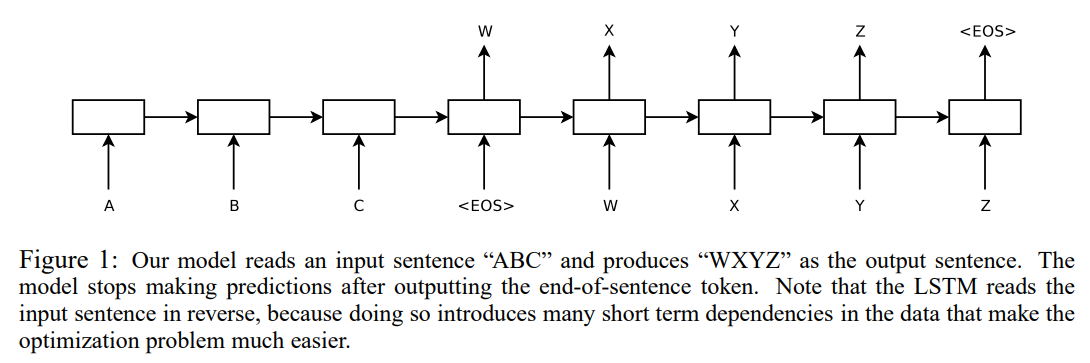
\includegraphics[width = 11cm]{figure/seq2seq.png}\\ 
	\beamergotobutton{\href{https://arxiv.org/pdf/1409.3215.pdf}{Source: Sutskever et al., 2014}}
	\end{figure}

\textbf{Used for:}

\begin{itemize}
	\item (Neural) Machine Translation
	\item Summarization
	\item Questions answering
\end{itemize}

\vfill

\end{vbframe}

% ------------------------------------------------------------------------------

\begin{vbframe}{benchmarking: traditional nlu}

\vfill

\begin{itemize}
	\item Nine sentence- or sentence-pair language understanding tasks
	\item Public leaderboard, (still) very popular benchmark collection
\end{itemize}

	\begin{figure}
		\centering
		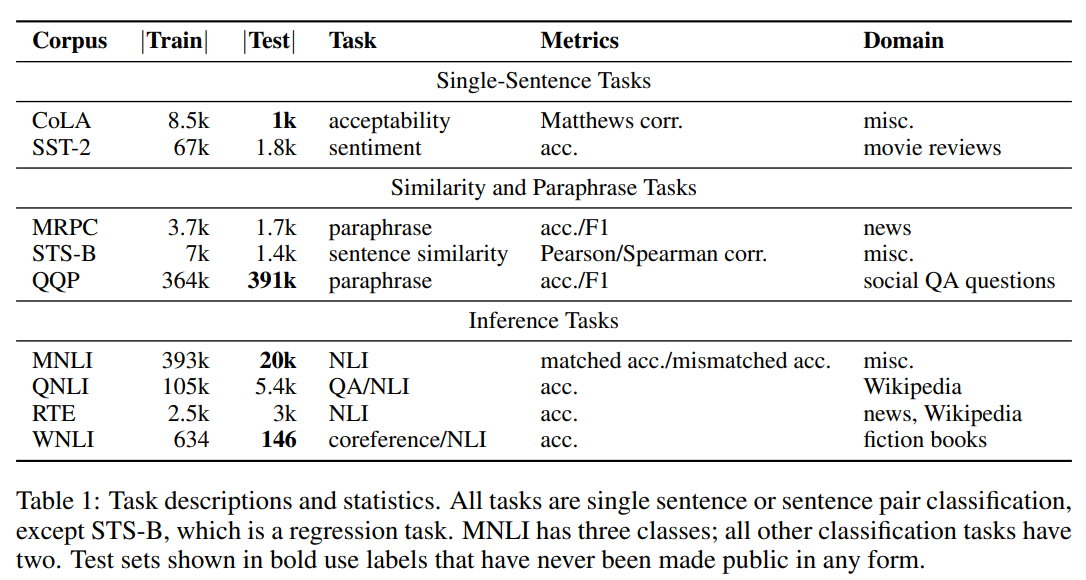
\includegraphics[width = 11cm]{figure/glue.png}\\ 
	\beamergotobutton{\href{https://openreview.net/pdf?id=rJ4km2R5t7}{Source: Wang et al., 2018}}
	\end{figure}

\vfill

\end{vbframe}

% ------------------------------------------------------------------------------

\begin{vbframe}{benchmarking: generation}

\vfill

\begin{itemize}
	\item \textbf{WinoGrande} 
	\begin{figure}
		\centering
		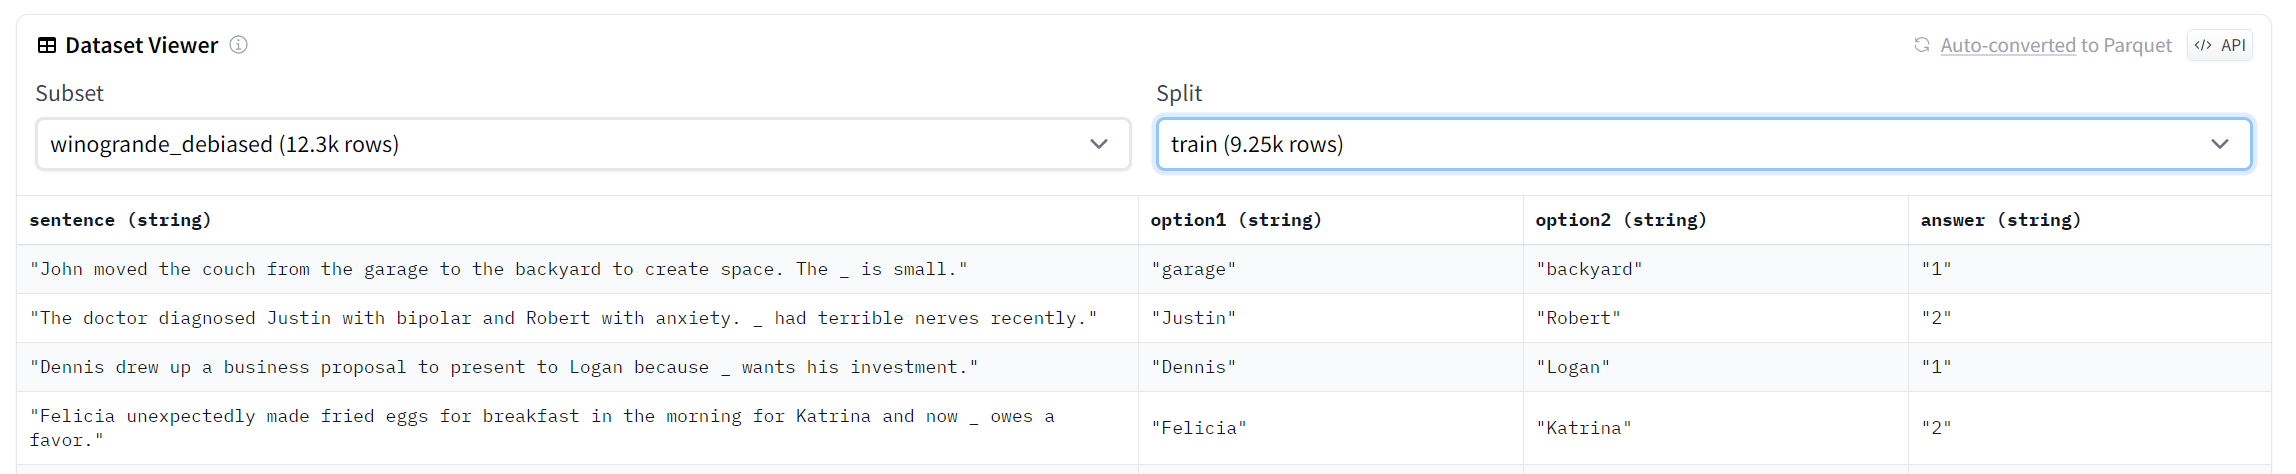
\includegraphics[width = 10cm]{figure/winogrande.png}\\ 
	\beamergotobutton{\href{https://arxiv.org/abs/1907.10641}{Source: Sakaguchi et al., 2019}}
	\end{figure}
	\item \textbf{HellaSwag} 
	\begin{figure}
		\centering
		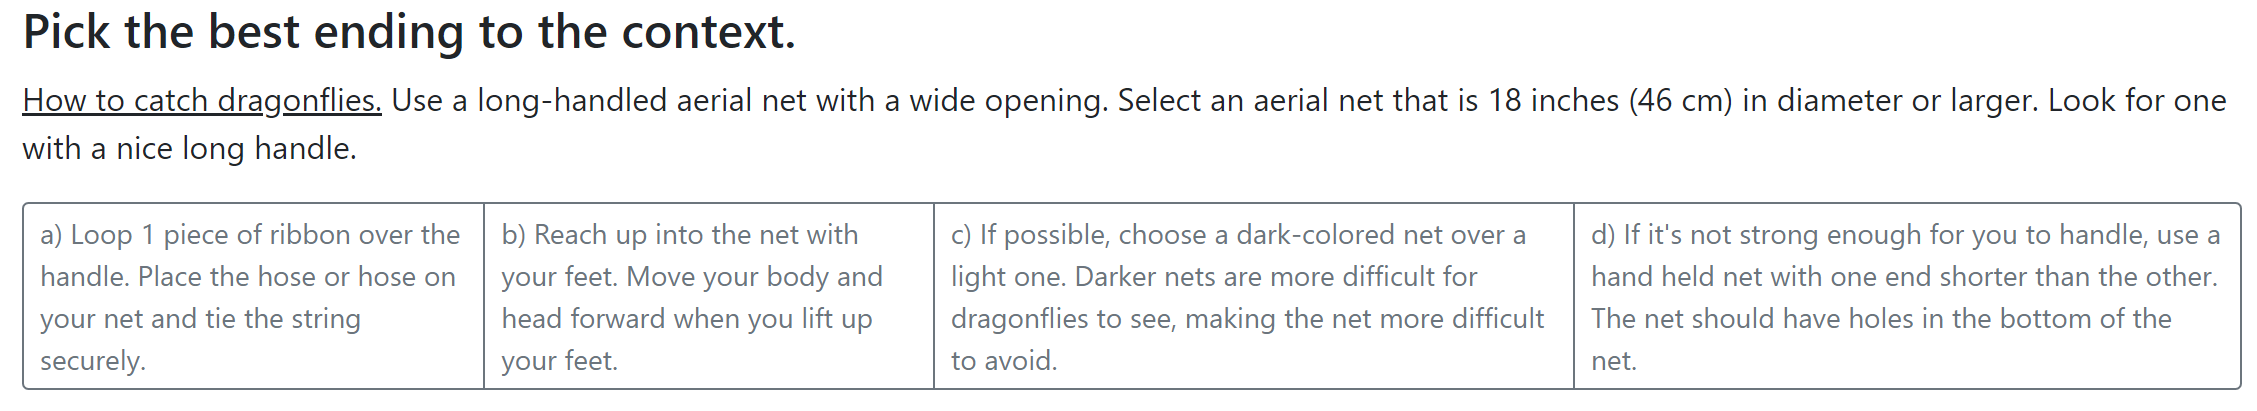
\includegraphics[width = 10cm]{figure/hellaswag.png}\\ 
	\beamergotobutton{\href{https://arxiv.org/abs/1905.07830}{Source: Zellers et al., 2019}}
	\end{figure}
\end{itemize}

\vfill

\end{vbframe}

% ------------------------------------------------------------------------------

\begin{vbframe}{benchmarking: generation}

\vfill

\begin{itemize}
	\item \textbf{LAMBADA}
	\begin{figure}
		\centering
		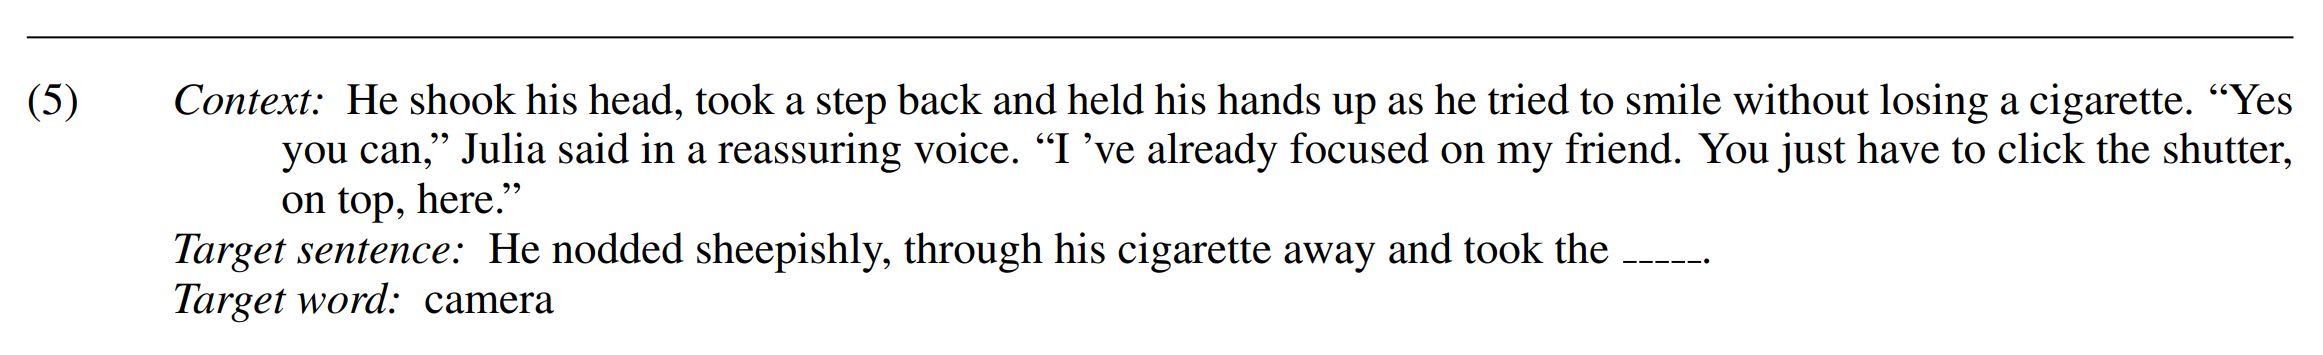
\includegraphics[width = 9cm]{figure/lambada.png}\\ 
	\beamergotobutton{\href{https://aclanthology.org/P16-1144/}{Source: Paperno et al., 2016}}
	\end{figure}
	\item \textbf{PIQA}
	\begin{figure}
		\centering
		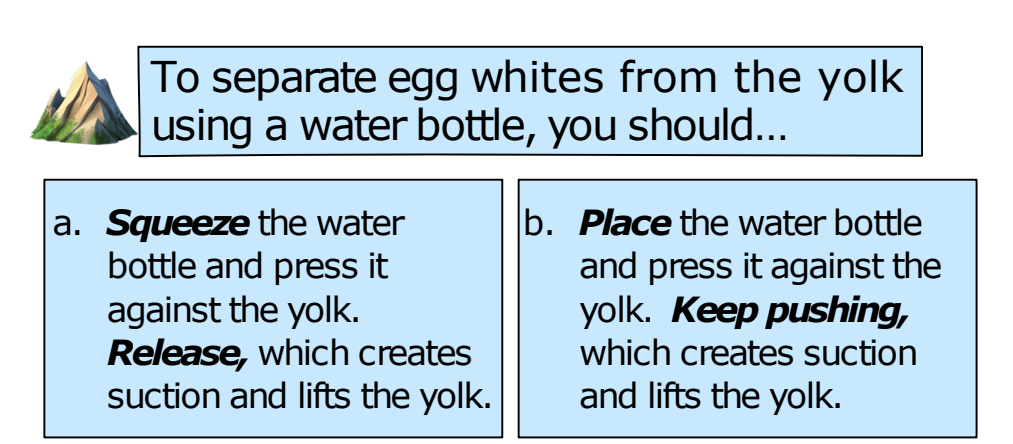
\includegraphics[width = 9cm]{figure/piqa.png}\\ 
	\beamergotobutton{\href{https://arxiv.org/abs/1911.11641}{Source: Bisk et al., 2019}}
	\end{figure}
\end{itemize}

\vfill

\end{vbframe}

% ------------------------------------------------------------------------------

\endlecture
\end{document}


% ------------------------------------------------------------------------------

\begin{vbframe}{benchmarking: traditional nlu}

\vfill

\begin{itemize}
	\item \textbf{CoLa}
	\begin{itemize}
		\item Short for "Corpus of Linguistic Acceptability"
		\item Binary classification: Linguistically acceptable or not
	\end{itemize}
	\item \textbf{SST-2 (Stanford Sentiment Treebank)} 
	\begin{itemize}
		\item Movie reviews annotated with their sentiment (pos/neg)
		\item Also available in a more fine-grained fashion (SST-5)
	\end{itemize}
	\item \textbf{MRPC (Microsoft Research Paraphrase Corpus)}
	\begin{itemize}
		\item Sentence pairs; Classify whether the are semantically equivalent
	\end{itemize}
	\item \textbf{QQP (Quora Question Pairs)} 
	\begin{itemize}
		\item Sentence pairs; Classify whether the are semantically equivalent
		\item Here: Questions (as opposed to "news" in MRPC)
	\end{itemize}
\end{itemize}

\vfill

\end{vbframe}

% ------------------------------------------------------------------------------

\begin{vbframe}{benchmarking: traditional nlu}

\vfill

\begin{itemize}
	\item \textbf{STS-B (Semantic Textual Similarity Benchmark)}
	\begin{itemize}
		\item Regression task (similarity score from 1 to 5)
	\end{itemize}
	\item \textbf{MNLI (Multi-Genre Natural Language Inference)} 
	\begin{itemize}
		\item Textual Entailment: Premise and Hypothesis are given
		\item Target: \textit{entailment / contradiction / neutral}
	\end{itemize}
	\item \textbf{QNLI (Stanford Question Answering Dataset)}
	\begin{itemize}
		\item Modified original task to binary classification
	\end{itemize}
	\item \textbf{RTE (Recognizing Textual Entailment)} 
	\begin{itemize}
		\item Collapsed to a binary classification task 
	\end{itemize}
	\item \textbf{WNLI (Winograd Schema Challenge)} 
	\begin{itemize}
		\item Coreference resolution task
		\item Rephrased to entailment task by providing the model with original sentence and sentence with the pronoun  
	\end{itemize}
\end{itemize}

\vfill

\end{vbframe}


% ------------------------------------------------------------------------------

\begin{vbframe}{Examples of low-level NLP tasks}

\textbf{Sequence tagging}

\begin{itemize}
	\item POS-tagging (part of speech)
\end{itemize}

\textbf{Structure prediction}

\begin{itemize}
	\item Chunking/Parsing
\end{itemize}

\textbf{Semantics}

\begin{itemize}
	\item Word sense disambiguation
\end{itemize}

\textbf{Morphological analysis}

\begin{itemize}
	\item Case Marker Extraction
\end{itemize}


	\begin{exampleblock}{Example}

	\end{exampleblock}
	
\vfill

\end{vbframe}
